\section{Introduction}
The Internet of Things (IoT), is a network of interrelated devices that connect and exchange data with other IoT devices and the cloud\cite{iot_techtarget}. These typse of devices are typically embedded with technology such as sensors and software, and can include mechanical and digital machines and consumer objects. They encompass everything from everyday household items to complex industrial tools, making the IoT sector one of the fastest-growing industries today.

With IoT, data is transferable over a network without requiring human-to-human or human-to-computer interactions. In its simplest term, IoT is perceived as a network of billions of devices that can sense, actuate and relay the information to a centralized system. IoT systems gather data from the sensors embedded in IoT devices, which is then transmitted through an IoT gateway for analysis by an application or back-end system. They represent the convergence of Information Technology (data processing and networking) with Operational Technology (hardware and software that detects or causes change through the direct monitoring and/or control of physical devices). The following diagram shows the workflow and the different components that can compose an IoT system. 

\begin{figure}[H]
	\centering
	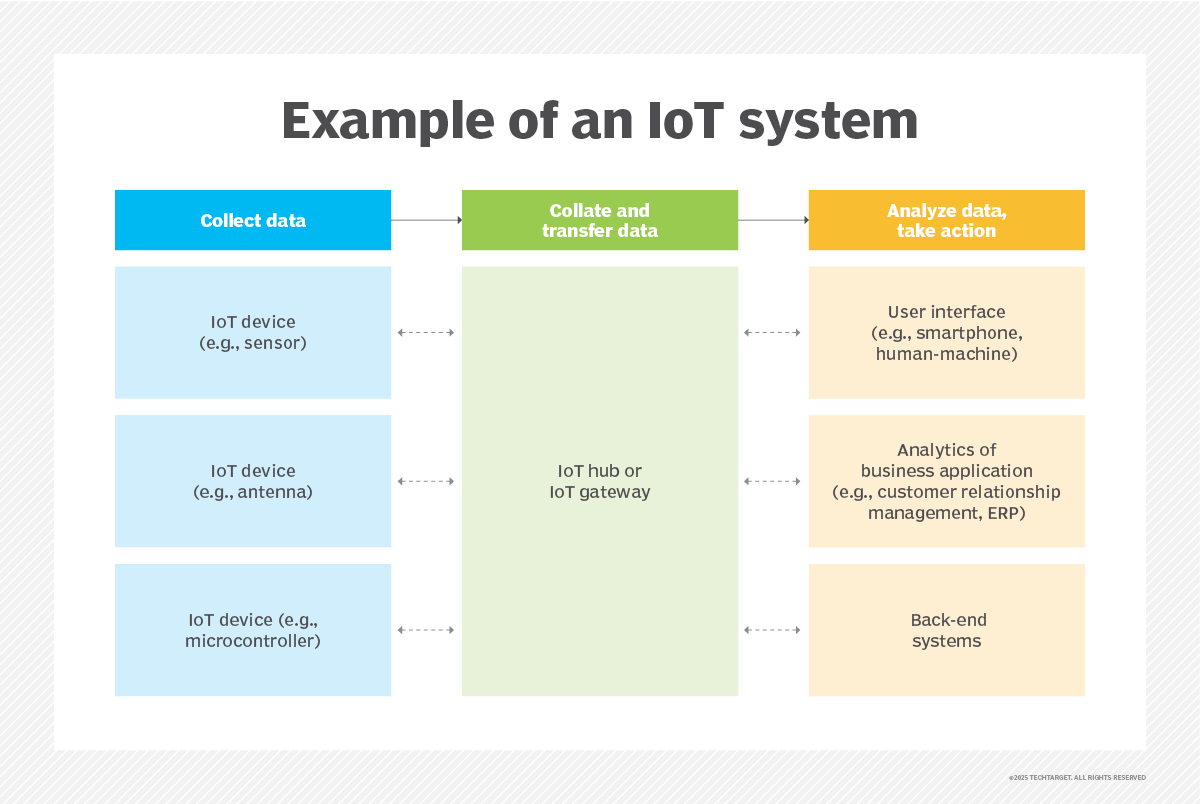
\includegraphics[width=0.7\linewidth]{../Images/introduction/iota-iot_system.png}
	\caption{Diagram of an Example IoT System \cite{iot_techtarget}}
	\label{fig:iota-industryiotsystem}
\end{figure}

As a result, the Internet has transitioned from joining end-user nodes to interconnecting physical objects, resulting in a more intelligent object network capable of insightful collaboration and intelligent processing \cite{Javaid2022}. The capabilities of these type of devices are many such as: 

\begin{itemize}
	\item \textbf{Sensing and Actuation:} Devices act as the "edge" between the digital and physical world, either collecting physical data (sensors like temperature or motion detectors) or altering the physical environment (actuators like smart locks or light switches).
	\item \textbf{Computation:} The devices have on-boarded computational power which allow them to perform data handling before transmitting it to reduce the volume of data sent to the cloud. 
	\item \textbf{Communication:} They use a network stack, normally low power protocols, to support many-to-many relationships, communicating either device-to-device or device-to-cloud.
	\item \textbf{Autonomy:} They are designed to monitor, automate, and trigger decisions with minimal to no human intervention. 
 \end{itemize}
 
 While these capabilities lead to unprecedented efficiency, they also drastically expand the attack surface. Their rapid proliferation has made them frequent targets for cybercriminals, transforming them into a critical and complex focal point for modern digital investigations.

\subsection{Context}
The widespread adoption of IoT systems has outpaced the implementation of robust security standards, introducing significant vulnerabilities into both consumer and enterprise environments. The Open Worldwide Application Security Project (OWASP) identifies several critical security challenges inherent to the IoT ecosystem \cite{OWASPIoT2018}. These challenges include among them: 

\begin{itemize}
	\item \textbf{Weak, Guessable or Hardcoded Passwords:} Devices are frequently shipped with publicly known default credentials that cannot be easily changed by the end user.
	
	\item \textbf{Insecure Network Services:} Unnecessary or vulnerable network services running on the device can expose the device to unauthorized access and packet sniffing.
	
	\item \textbf{Lack of Secure Update Mechanisms:} Many devices the ability to receive firmware updates, or to validate update files cryptographically leaving them permanently vulnerable to discovered exploits. 
	
	\item \textbf{Insecure Data Transfer and Storage:} The lack of strong encryption at rest or in transit allows sensitive operational data to be intercepted or manipulated. 
\end{itemize}

Because of these pervasive security flaws, IoT devices are increasingly weaponized in cyberattacks, serving as entry points for lateral network movement, nodes in distributed denial-of-service (DDoS) botnets, or tools for data exfiltration. Consequently, these devices hold immense forensic value. 

\subsection{Digital Forensic Problems with IoT}

Nevertheless, extracting evidence from these devices exposes the severe inadequacy of traditional digital forensic methodologies. Traditional computer forensics rely on a "dead-box" analysis, a process where the investigator can isolate the device, clone its storages media and then analyse the file system and system logs \cite{NISTSP80086}.

IoT devices are totally opposite to this approach. They rely on proprietary hardware, closed source custom firmware and rarely feature standardized physical interfaces such as SATA or USB ports that allow forensically data extraction. Furthermore, due to the necessity of minimizing manufacturing costs and power consumption, they are designed with constrained storage capacities. The vast majority of operational data, state information, and cryptographic keys are held in volatile memory (RAM) \cite{Alenezi2025}. If a device is rebooted, whether intentionally by a malicious actor or accidentally by a user, the evidence is permanently destroyed. Furthermore, even if logging exists on the device's flash memory, the severe storage limitations dictate that these logs are overwritten extremely rapidly in a continuous loop.

\subsubsection{Network Forensics}

Networked computing, wireless communications and portable electronic devices have expanded the role of digital forensics beyond traditional computer crime investigations  \cite{MacDermot2020}. Network Forensics  techniques  assist  in tracking internal  and external  network  attacks  by focusing on the devices present and the communication mechanisms applied. The purpose of such an analysis is to explore digital evidence in the network traffic after the occurrence of a suspicious event. In a larger scale environment, it is the ability to sift through gigabytes of the captured network traffic and construct multiple views of that traffic benefits network security, policy enforcement, and network maintenance personnel. For all these reasons, Cloud Forensics is an emerging branch of Network Forensics.

The objective is the same as physical crime scenes, determining the crime, identifying and analysing the evidence the evidence and establishing the party or parties involved. As for now, there is a standardised method for retrieving evidence from traditional devices but no clear procedures for IoT based investigations, which will require a multi-faceted approach. 

iveGn that the IoT devices usually act as inaccessible black boxes with fleeting data, investigators are forced to seek alternative sources of evidence. The defining characteristic of any IoT device is its connectivity, which makes the network traffic it generates its main artefact from where to extract evidence. This traffic is normally easy to analyse since they are single-purpose machines whose patterns are highly predictable and structured. 

However, applying traditional network forensics to IoT environments introduces significant technical challenges:

\begin{itemize}
	\item \textbf{Encrypted Payload Barrier:} To protect the user privacy, modern IoT protocols employ encryption techniques. This renders Deep Packet Inspection obsolete. Investigators must rely entirely on encrypted metadata, such as flow duration, inter-arrival times (IAT) and packet lengths. 
	\item \textbf{Blurry Network Boundaries:} Not correctly defined perimeter edges in the network are an issue for IoT investigations. The location of evidence effects ease of access, possible connections to other devices (local or cloud based), etc. 
	\item \textbf{Time Synchronization:} The existence of multiple sources presents the possibility of different time zone refereces, timestamp interpretations, clock drift issues which can all impact to the ability of generating a unified timeline\cite{Lillis2016}.
	\item \textbf{Semantic gap in Behavioral Translation:} There is a disconnection between raw network data and physical device actions. It is highly complex to map a specific encrypted TCP flow to a real-world event, such as trying to distinguish if a smart lock's network spike indicates a legitimate user unlocking the door or an attacker brute forcing the credentials. 
	\item \textbf{Volume and Background Noise:} IoT devices are constantly generating background traffic such as keep-alive messages, heartbeat signals to cloud servers and NTP time synchronizations. Filtering this benign ambient noise to isolate the exact packets corresponding to a forensic event is a major analytical hurdle. 
\end{itemize}


\subsection{Motivation}
Motivated by these specific challanges, specially the volatility of device-level evidence and the semantic gap present in encrypted communications, this project focuses on developing a robust methodology for IoT behavioral reconstruction. This research aims to validate how passive network forensics can be used to infer physical device actions, bridging the gap between raw network metadata and actionable forensic intelligence. 


\subsection{Objectives}
The main objective of this project is to establish and validate a robust methodology for the behavioral reconstruction of IoT devices using passive network forensics. Due to the previously introduced challenges and limitations, this research focuses on leveraging network evidence to bridge the semantic gap between raw traffic and physical device actions. To achieve this, the project is designed to directly address the following research questions: 

\begin{enumerate}
	\item \textbf{Can IoT device activity be inferred solely from network traffic?} By analyzing encrypted packet flows, this project will determine the extent to which physical device actions can be deduced without accessing local device storage. 
	\item \textbf{Which network features best identify device behaviour?} The research will evaluate various traffic metrics such as packet lengths, flow durations, inter-arrival times and specific protocol usage to identify the most reliable indicators if distinct device states. 
	\item \textbf{How accurately can forensic timelines be reconstructed?} By comparing inferred network events against a known baseline of simulated attacks, the project will measure the precision of network-based timeline reconstruction. 
\end{enumerate}

To be able to answer these questions, the development of the project is structured around the following actionable objectives: 

\begin{itemize}
	\item \textbf{Environment Simulation:} Create a simulated smart home network utilizing virtual IoT devices and lightweight device emulators to generate realistic operational traffic. 
	
	\item \textbf{Threat Simulation and Data Capture:} Establish a baseline of typical device operations, and simulate specific cyberattacks while capturing comprehensive network traffic traces.
	
	\item \textbf{Feature Extraction and Packet Analysis:} Process the captured traffic abd isolate the behavioural network features using network monitoring tools.
	
	\item \textbf{Behavioural Classification and Methodology Design:} Develop a clear classification of IoT device behaviors based on their network footprints, and formulate a step-by-step methodology for investigators conducting network-based IoT forensics.
	
	\item \textbf{Dataset Contribution:} Curate, document, and package the generated network traffic traces into an experimental dataset to be utilized for future IoT forensic research and validation.
\end{itemize}

\subsection{Scope and Limitations}
To ensure the feasibility and academic rigor of this research, clear boundaries have been established regarding the environment, methodologies, and technologies evaluated.

\subsubsection{Scope}
This project strictly focuses on the passive network forensic analysis of IoT environments. The boundaries of the research are defined as follows:
\begin{itemize}
	\item \textbf{Simulated Environment:} The practical experimentation will be conducted within a controlled, simulated smart home network topology. This environment will be constructed using lightweight device emulators and virtualization tools to represent common IoT nodes, such as smart cameras, sensors, and smart plugs.
	\item \textbf{Traffic Analysis:} The research relies entirely on passive network traffic capture and analysis. The extraction of forensic artifacts will be performed using standard network parsing tools, specifically on metadata rather than payload content.
	\item \textbf{Threat Scenarios:} The behavioral reconstruction will focus on a predefined set of common IoT threat scenarios, specifically targeting unauthorized accessand anomalous data flows.
	\item \textbf{Deliverables:} The project will yield a step-by-step forensic methodology, a classification of device behaviors based on network features, and an experimental log dataset generated from the simulated environment.
\end{itemize}

\subsubsection{Limitations}
While the simulated approach allows for a highly controlled experimental dataset, it inherently introduces certain limitations to the research:

\begin{itemize}
	\item \textbf{Emulation vs Physical Hardware:} Since the project utilizes virtualized devices and emulators, the generated traffic may lack the complete proprietary background noise and undocumented telemetry that commercial IoT devices present in the real world.
	\item \textbf{Exclusion of Device and Cloud Forensics:} This research operates strictly at the network layer. It explicitly excludes device-level "dead-box" forensics (e.g., memory dumping) as well as cloud forensics (e.g., acquiring data from a vendor's backend).
	\item \textbf{Encrypted Payloads:} The methodology assumes that modern IoT traffic is encrypted (e.g., TLS/SSL). Therefore, the project does not attempt to break encryption, decrypt traffic, or perform Deep Packet Inspection (DPI) on payload data. All inferences are derived from encrypted traffic analysis and flow metadata.
	\item \textbf{Network Scale:} The simulated smart home represents a small-scale, localized network. The findings and the volume of background noise may not directly scale to massive, enterprise-level Industrial IoT (IIoT) deployments or smart city infrastructures.
\end{itemize}

